\documentclass{article}
\usepackage[utf8]{inputenc}
\usepackage[spanish]{babel}
\usepackage{graphicx}
\graphicspath{ {images/} }

\usepackage{listings}
\lstdefinestyle{code}{
language=Octave,
frame=single,
breakatwhitespace=true,
breaklines=true,
basicstyle=\small\ttfamily,
tabsize=4,
numbers=left,
numberstyle=\tiny,
columns=fullflexible
}
\lstdefinestyle{snippet}{
language=Octave,
breakatwhitespace=true,
breaklines=true,
basicstyle=\small\ttfamily,
}

\addtolength{\textwidth}{1cm}

\title{Práctica 0}
\author{Héctor Laria Mantecón y Samuel Lapuente Jiménez}
\date{15 de octubre de 2015}

\begin{document}

\maketitle
\section{Introducción}
Dada una función real e integrable de una sola variable, se ha utilizado 
el método de {\it Monte Carlo} descrito en el guión de la práctica para 
calcular su integral entre dos puntos.

Se han implementado dos funciones, {\tt mcint\_iterativo}, que hace 
tantas vueltas como puntos se generan y {\tt mcint\_vector}, que utiliza 
vectores para hacer los cálculos.

\section{Desarrollo}
Se utiliza la función $f(x) = x^2$ entre los valores $-6$ y $6$ y cuya 
integral según {\tt quad} es $144$ para probar la exactitud de los 
métodos.

\subsection{Versión iterativa}
El código es el siguiente:
\lstinputlisting[style=code]{src/mcint_iterativo.m}

La función nos da una integral de $142.00$ unidades con un ejemplo de 
ejecución de $10000$ puntos aleatorios, representados en esta gráfica:
\begin{figure}[h]
\centering
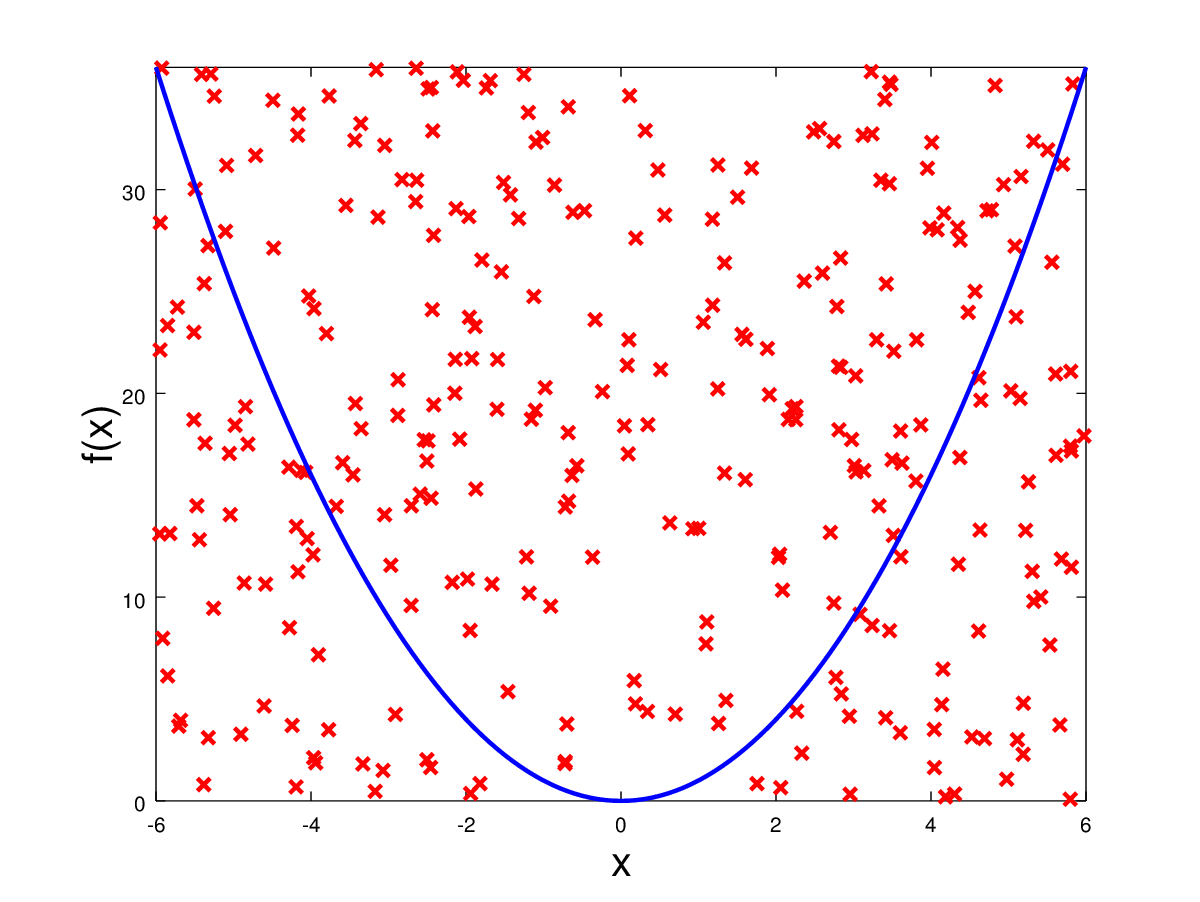
\includegraphics[width=12cm]{iterativo}
\end{figure}

Para calcular el tiempo que tarda en hacer el cálculo, introducimos en 
el intérprete:
\begin{lstlisting}[style=snippet]
>> tic(); mcint_iterativo(@(x) (x.^2), -6, 6, 10000); time = toc()
\end{lstlisting}
Que nos da una respuesta de {\tt time =  0.26014} segundos.

\subsection{Versión con vectores}
Para la versión usando vectores hacemos:
\lstinputlisting[style=code]{src/mcint_vector.m}

Nos da una integral de $144.59$ unidades con la misma cantidad de 
puntos, distribuidos en esta ejecución:
\begin{figure}[h]
\centering
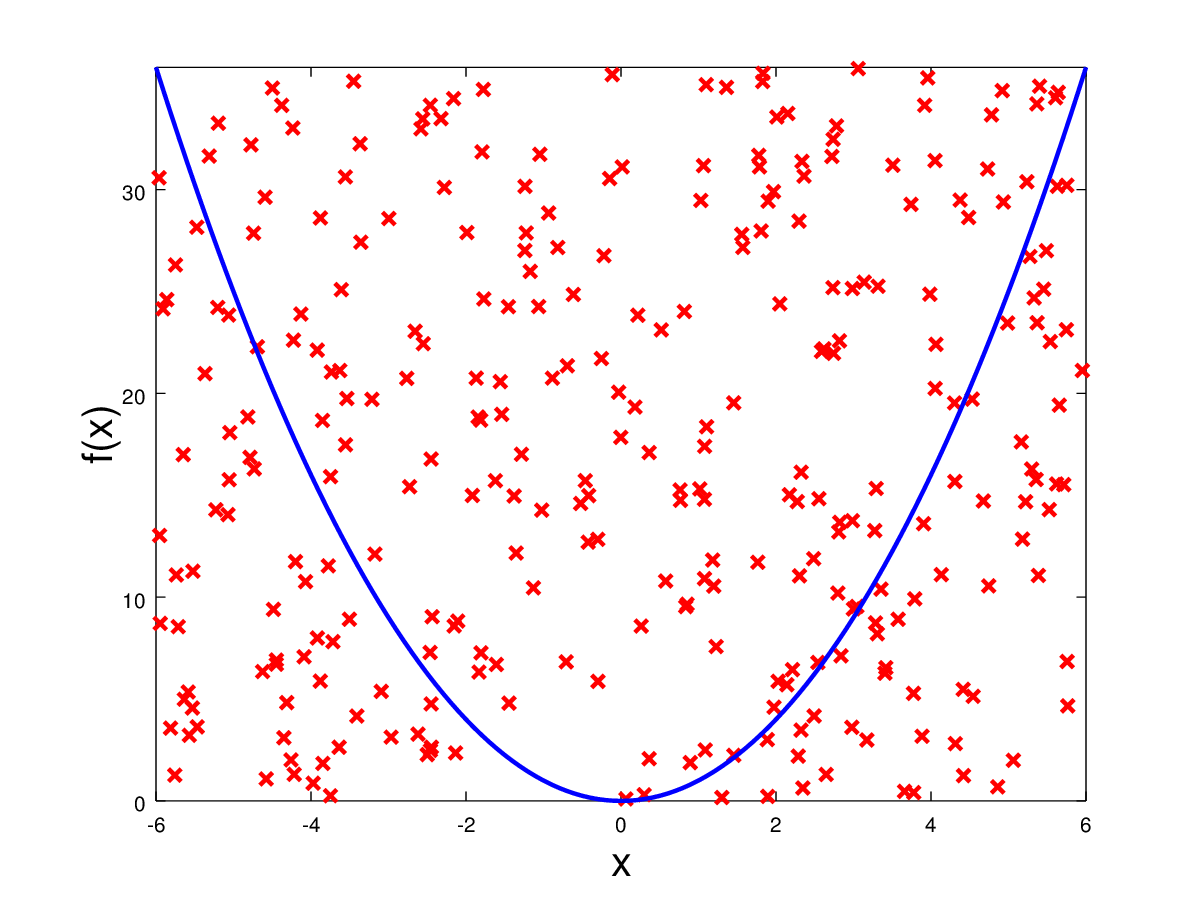
\includegraphics[width=12cm]{vector}
\end{figure}
En un tiempo {\tt time =  0.095317}.
\pagebreak

\subsection{Parte opcional}
Como parte opcional en el laboratorio, se pedía un script que pintara la 
aproximación de una de las anteriores funciones dependiendo del número 
de puntos aleatorios que se generaban para calcular la integral.

Para la función anterior sale esta gráfica:
\begin{figure}[h]
\centering
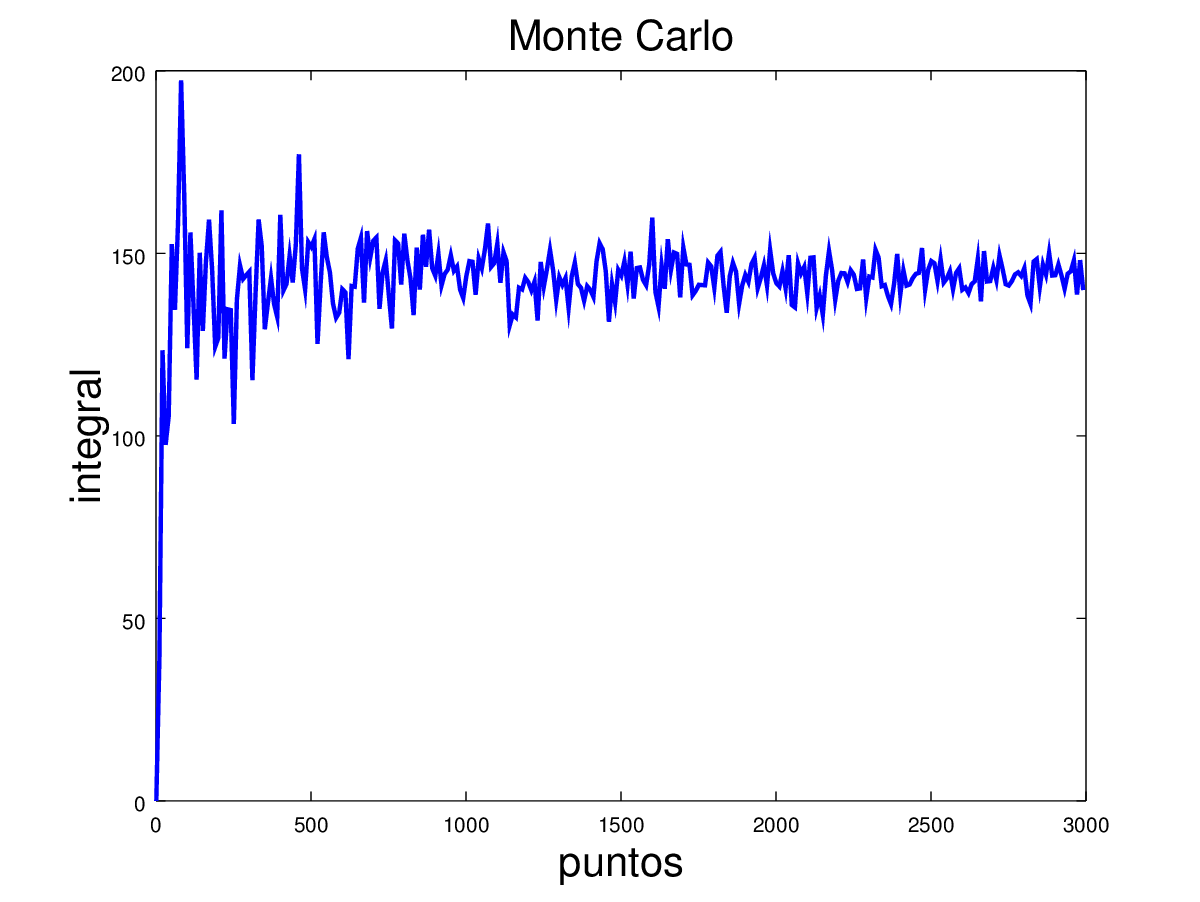
\includegraphics[width=12cm]{estudio}
\end{figure}

Generada con este código:
\lstinputlisting[style=code]{src/estudio.m}

\section{Conclusión}
La realización de la práctica nos da a concluir que en {\it Octave} el 
cómputo es mucho más rápido cuando se hace con operaciones sobre 
vectores que con bucles, siendo la diferencia de $2.7$ veces mejor y 
aumentando considerablemente cuanto mayor es el tamaño del problema, 
llegando en esta práctica a dar datos de más de $200x$.

\end{document}
